%!TEX root = ../thesis.tex

\section{実験目的}
シミュレータ上で実験を行い, 提案手法の有効性を検証する.

\section{実験装置}
実験は, \figref{Fig:gazebo}に示すGazebo\cite{gazebo}のWillow Garage\cite{willow}で\figref{Fig:willow-garage}に示すコースで一周行う. また, ロボットモデルには\figref{Fig:turtlebot3}に示すようなカメラを3つ搭載したTurtlebot3\cite{turtlebot3}を用いた. 

\begin{figure}[h]
  \centering
  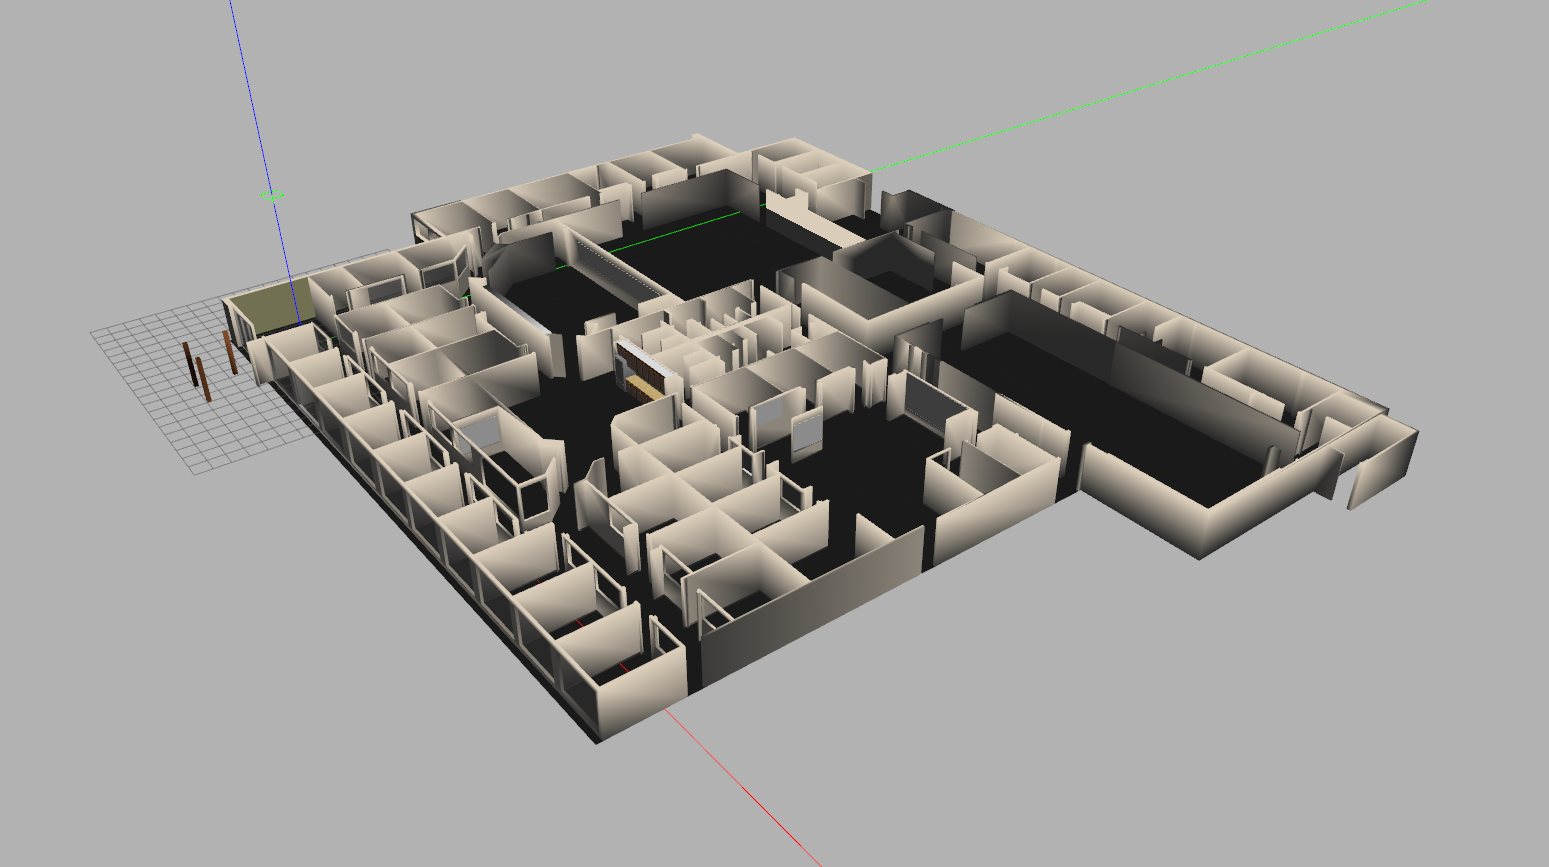
\includegraphics[keepaspectratio, scale=0.15]{images/gazebo.png}
  \caption{Experimental environment in simulator}
  \label{Fig:gazebo}
  \end{figure}

\newpage
\vspace{20mm}
\begin{figure}[h]
  \centering
  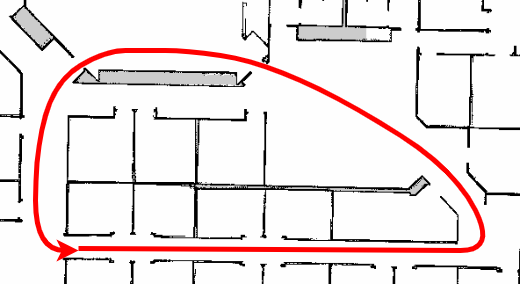
\includegraphics[keepaspectratio, scale=0.5]{images/willow-path.png}
  \caption{Course to collect data}
  \label{Fig:willow-garage}
  \end{figure}

\begin{figure}[h]
  \centering
  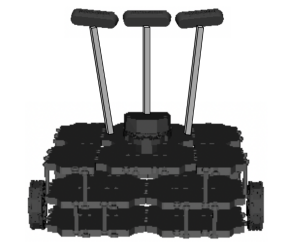
\includegraphics[keepaspectratio, scale=0.55]{images/turtlebot3.png}
  \caption{Turtlebot3 waffle with 3 cameras}
  \label{Fig:turtlebot3}
  \end{figure}

\newpage
\section{実験方法}
\begin{description}
  \item[1)データ収集]\mbox{}\\データの収集方法について述べる. \figref{Fig:old-method}にデータの収集方法を示す. 図のようにロボットを目標経路上と目標経路から±0.1[m], ±0.2[m], ±0.3[m]の位置に配置する. 位置に関する実験条件は, 以下の4種類となる. 
  \par (a)目標経路上のみ
  \par (b)目標経路上と目標経路から±0.1[m]の位置
  \par (c)目標経路上と目標経路から±0.2[m]の位置
  \par (d)目標経路上と目標経路から±0.3[m]の位置
  \vskip\baselineskip
  \par また, 各位置において, 目標経路の向きを基準として, ロボットをヨー方向に0[deg]と±5[deg]回転させる. 角度に関する実験条件は, 以下の2種類となる. 
  \par (e)目標経路の向きと±5[deg]回転させた向き
  \par (f)目標経路の向きのみ
\end{description}

\begin{figure}[h]
  \centering
  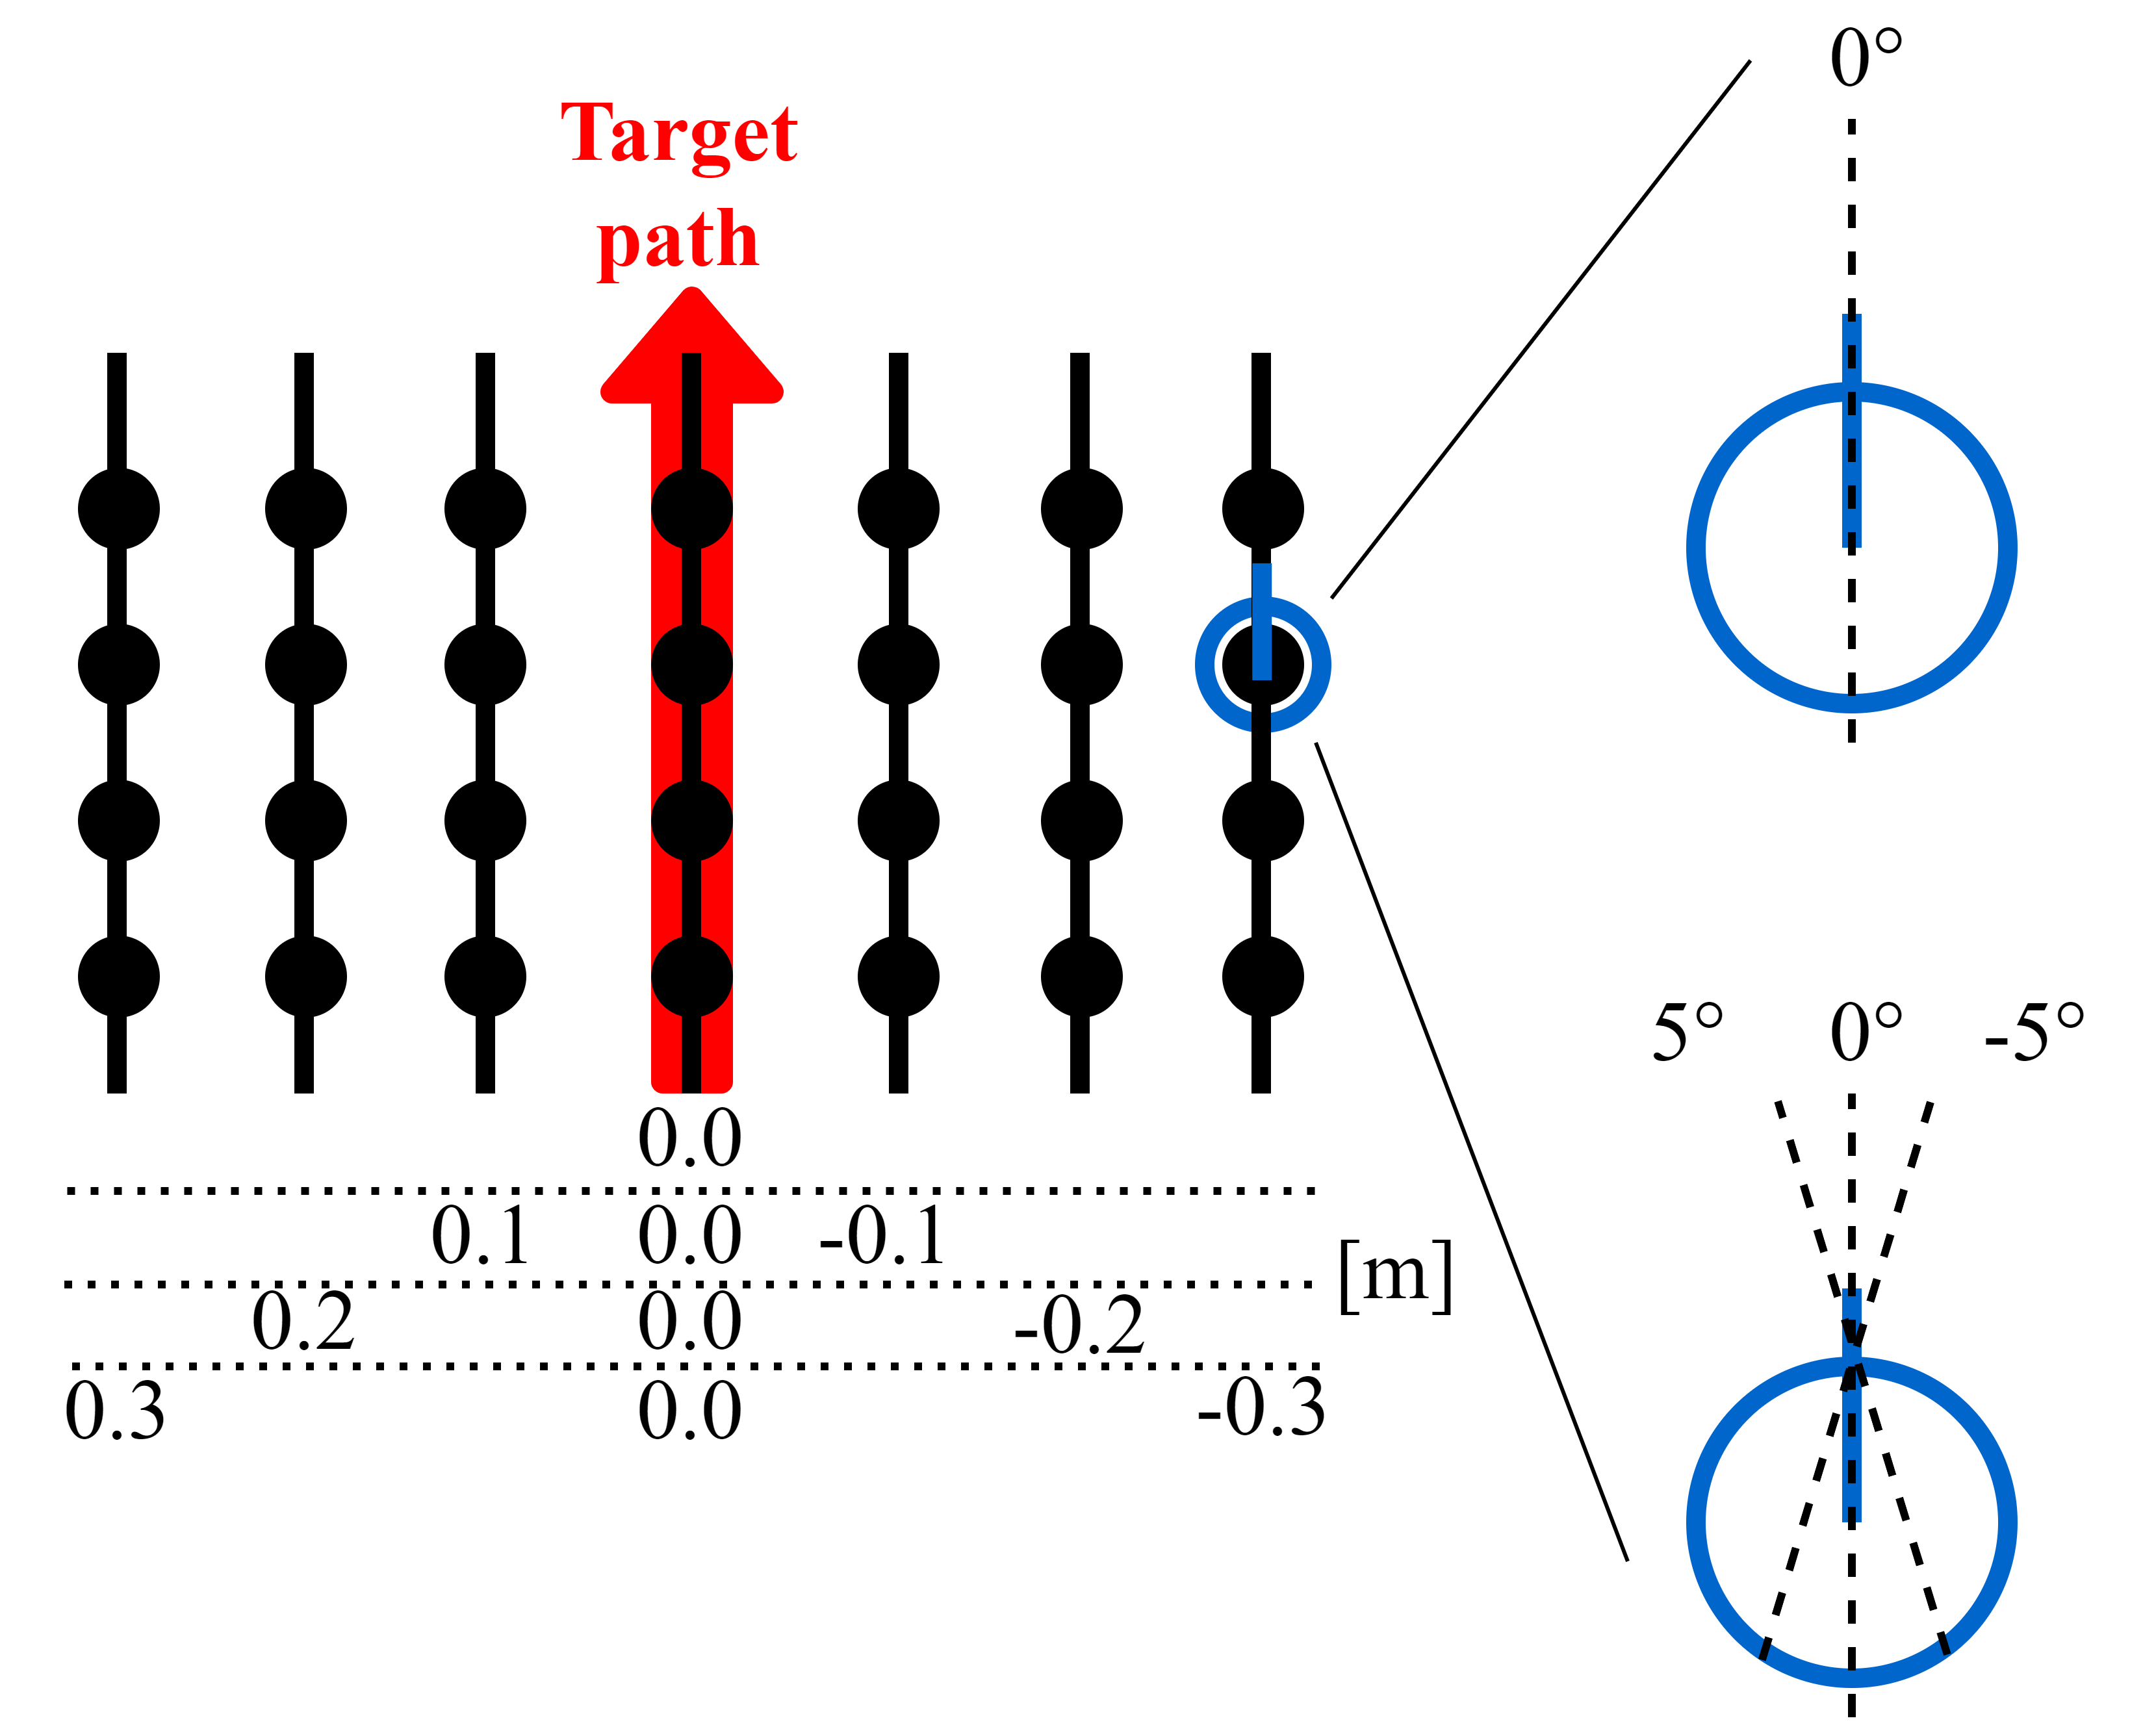
\includegraphics[keepaspectratio, scale=0.6]{images/collect2.png}
  \caption{Location and orientation of the robot in the experiments}
  \label{Fig:old-method}
  \end{figure}

\begin{description}
  \item[2)訓練]\mbox{}\\収集したデータ2を用いて, バッチ学習を4000step行う. なお, オンライン手法では同様の条件で8000step行っていた. オフライン手法では, 後に述べるように4000stepでlossがほぼ収束するため, 4000stepを採用した.
\end{description}

\begin{description}
  \item[3)テスト]\mbox{}\\ 学習したモデルを用いてロボットを走行させ, \figref{Fig:willow-garage}に示した目標経路を追従できるかを検証する. ロボットの並進速度0.2m/sとし, 経路を1周できた場合を成功とし, 壁に激突した場合を失敗とした.
  \par 上記の2)学習と3)テストを30回行い, 経路追従の成功回数を求めた. 
\end{description}

\section{実験結果と考察}
実験結果を表\ref{tb:exp1}に示す. 列は位置の4条件(a)~(d)を並べたものであり, 行は方向の2条件(e), (f)を並べたものである. 分母の30は実験回数を示しており, 分子の数は成功回数を示している. 結果的に, 目標経路上及び±0.2[m]の位置, 0[deg]及び±5[deg]の向きに, ロボットを配置する条件で100%(30回中30回)成功している. これは, オンライン手法において最も高い成功率100%\cite{okada-si2021}と同じである. オンライン手法が40分程度必要なのに対して, オフライン手法での学習時間は4分程度であったことから, 学習に要する時間を1/10に短縮できることを確認できた. ただし, オフライン手法での学習時間4分には, 実験方法で述べたデータ収集は含まれていない. 

\begin{table}[h]
  \centering
  \caption{Number of successes in the batch learning}
  \begin{tabular}{|p{2cm}|p{2cm}|p{2cm}|p{2cm}|p{2cm}|} \hline
     & 0[m] & 0, ±0.1[m] & 0, ±0.2[m] & 0, ±0.3[m] \\ \hline
    0, ±5[deg] & 1/30 & 28/30 & \bf30/30 & 27/30 \\ \hline
    0[deg] & 0/30 & 14/30 & 23/30 & 20/30 \\ \hline
  \end{tabular}
  \label{tb:exp1}
\end{table}

ここで, \figref{Fig:loss_00_02_4000}に, この実験条件で学習したときのlossグラフを示す. 図から4000stepでlossがほぼ収束している様子が見られる. 

\newpage
\begin{figure}[h]
  \centering
  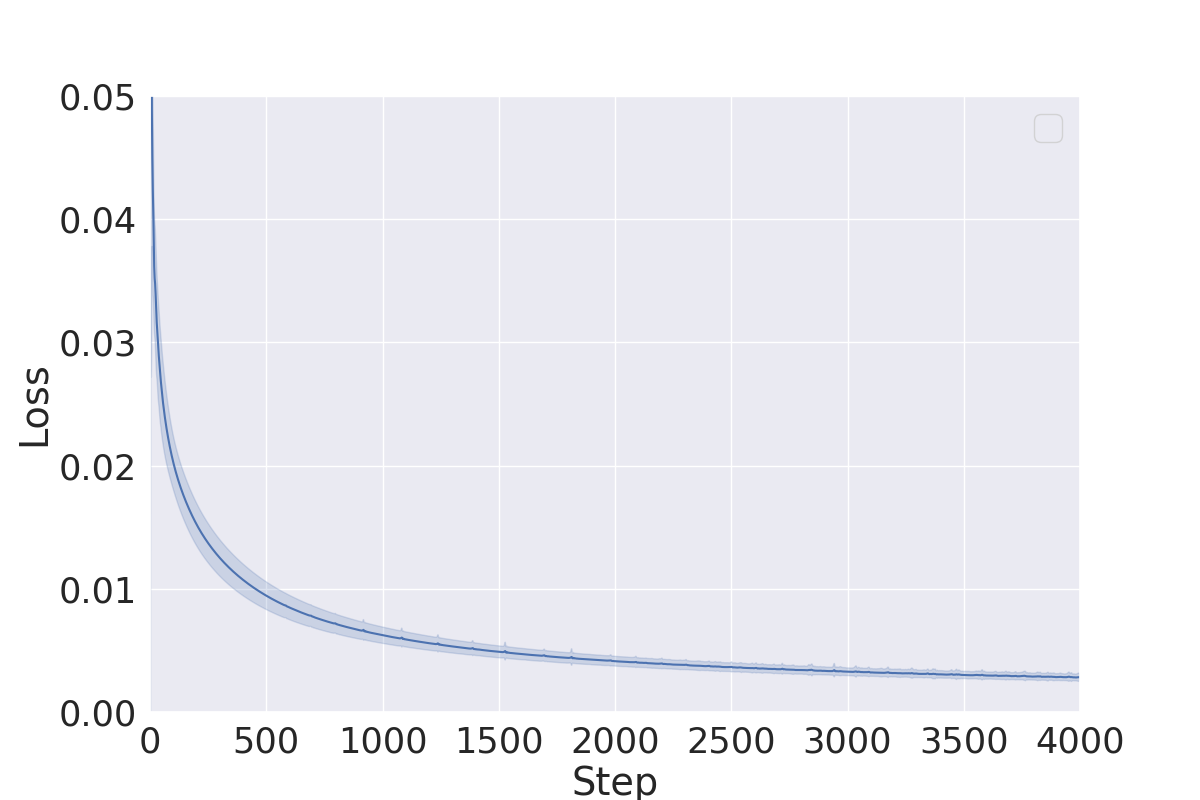
\includegraphics[keepaspectratio, scale=0.35]{images/loss_00_02_4000.png}
  \caption{Loss value in the experiment}
  \label{Fig:loss_00_02_4000}
  \end{figure}

また, \ref{tb:exp1}の他の結果を見ると, 30回成功した実験条件(位置0[m], ±0.2[m], 向き0[m], ±5[deg])から離れるほど成功率が低くなっている. 特にカメラの方向が0[deg]のみの場合は顕著に成功率
が低くなっている. また, 目標経路上の画像しか使用しない条件(位置0[m])では, ほとんど成功していない. それ以外の実験条件でも, カメラ間の距離により成功率が変化する様子が見られているが, この原因の究明は今後の課題としたい. 

\section{まとめ}